\paragraph{QuizziPedia::Front-End::Views\\::ShowAllCreatedQuestionnairesView}
\begin{figure} [ht]
	\centering
	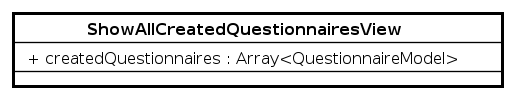
\includegraphics[scale=0.80]{UML/Classi/Front-End/QuizziPedia_Front-end_Views_ShowAllCreatedQuestionnairesView.png}
	\caption{QuizziPedia::Front-End::Views:ShowAllCreatedQuestionnairesView}
\end{figure} \FloatBarrier
\begin{itemize}
	\item \textbf{Descrizione}: \textit{view\ped{G}} per la visualizzazione dei questionari creati da un utente;
	\item \textbf{Utilizzo}: permette all'utente di visualizzare i questionari da lui creati;
	\item \textbf{Relazioni con altre classi}:
	\begin{itemize}
		\item \textbf{IN \texttt{ShowAllCreatedQuestionnairesModelView}}: classe di tipo modelview la cui istanziazione è contenuta all'interno della variabile di ambiente \texttt{\$scope} di \textit{Angular\ped{G}}. All'interno di essa sono presenti le variabili e i metodi necessari per il \textit{Two-Way Data-Binding\ped{G}} tra la \textit{view\ped{G}} \texttt{ShowAllCreatedQuestionnairesView} e il \textit{controller\ped{G}} \texttt{ShowAllCreatedQuestionnairesController};
		\item \textbf{IN \texttt{LangModel}}: rappresenta il modello delle informazioni per la giusta traduzione dell'applicazione.
	\end{itemize}
		\item \textbf{Attributi}:
		\begin{itemize}
			\item \texttt{+ createdQuestionnaires: Array<QuestionnaireModel>} \\ \texttt{array} contenente i questionari creati dall'utente loggato. 
		\end{itemize}
\end{itemize}